\chapter{WarpSpecialization for Blackwell}

\begin{center}\small 作者：CalebDu（知乎 @qi-qi-qi-qi-98-47）\quad 原文：\url{https://zhuanlan.zhihu.com/p/1941232816185644696}\end{center}

% 转换章内部放宽断行：原文含大量无自然断点的长标识符，避免 \hbox 溢出（只在本章生效）
\begingroup\setlength{\emergencystretch}{2em}

\section{前言：}

本文旨在结合cutlass的源码，学习一下blackwell 架构的GPU的新特性如何在cutlass中应用。本期的主题是Warp\allowbreak{}Specialization 在Blackwell 架构上的应用。参考的主要实现是include/\allowbreak{}cutlass/\allowbreak{}gemm/\allowbreak{}kernel/\allowbreak{}sm100\_\allowbreak{}gemm\_\allowbreak{}tma\_\allowbreak{}warpspecialized.hpp 和include/\allowbreak{}cutlass/\allowbreak{}gemm/\allowbreak{}collective/\allowbreak{}sm100\_\allowbreak{}mma\_\allowbreak{}warpspecialized.hpp，（不同的gemm实现的细节有差异）。

\section{WarpSpecialization：}

在先前的文章(\href{https://zhuanlan.zhihu.com/p/8488333314}{Nvidia Cute 实战-Warp\allowbreak{}Specialization Gemm} 和 \href{https://zhuanlan.zhihu.com/p/1905383022901059783}{Nvidia Cute 实战-Warp\allowbreak{}Specialization Gemm for Hopper}) 中，介绍了Hopper和Ampere架构上Gemm Warp\allowbreak{}Specialization(WASP) 的实现，简单的来说WASP的目的就是把复杂的指令流解耦，让warp负责各自解耦后的子任务，避免不同指令流之间的互相阻塞，使得warp scheduler更高的调度指令发射。

\begin{figure}[H]\centering
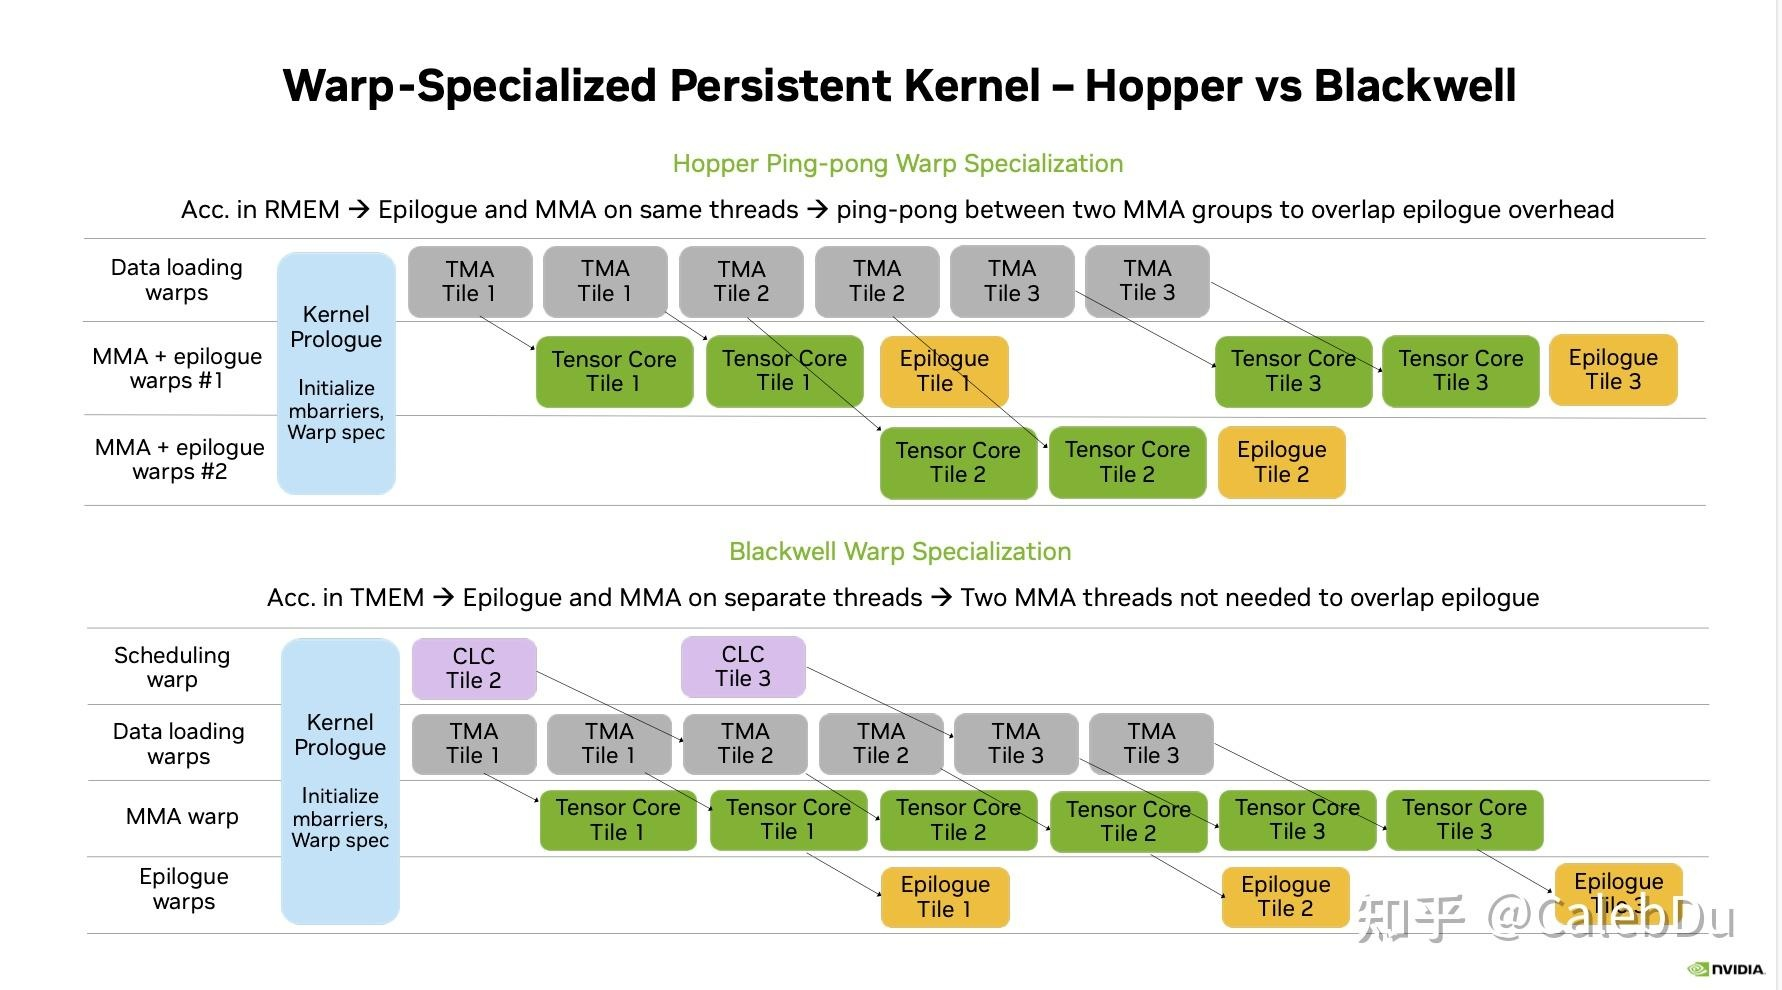
\includegraphics[width=\textwidth]{figures/calebdu-01-warp-specialization/fig-01.jpg}
\caption{Programming Blackwell Tensor Cores with CUTLASS GTC 25}
\end{figure}

在介绍Blackwell 的Warp\allowbreak{}Specialization 实现之前，我们先简单回顾一下Hopper上的WASP的实现，在Hopper上的WASP pingpong实现 launch 3个warp group(12个warp），一个warp group 中的两个warp作为生产者分别load mainloop和epilog 的数据，另外两个warp group作为消费者计算 生产者load的mainloop数据，通过tma pipeline进行生产者/\allowbreak{}消费者之间的同步。为了通过mainloop的tensorcore计算来掩盖epilog的操作，两个warp group之间利用sequence ordered pipeline来保证两个warp group mainloop/\allowbreak{}epilog 的overlap。以上的提到的pipeline 都是基于ptx mbarrier指令进行封装的，整一个WASP的核心也就是基于mbarrier。

\begin{figure}[H]\centering
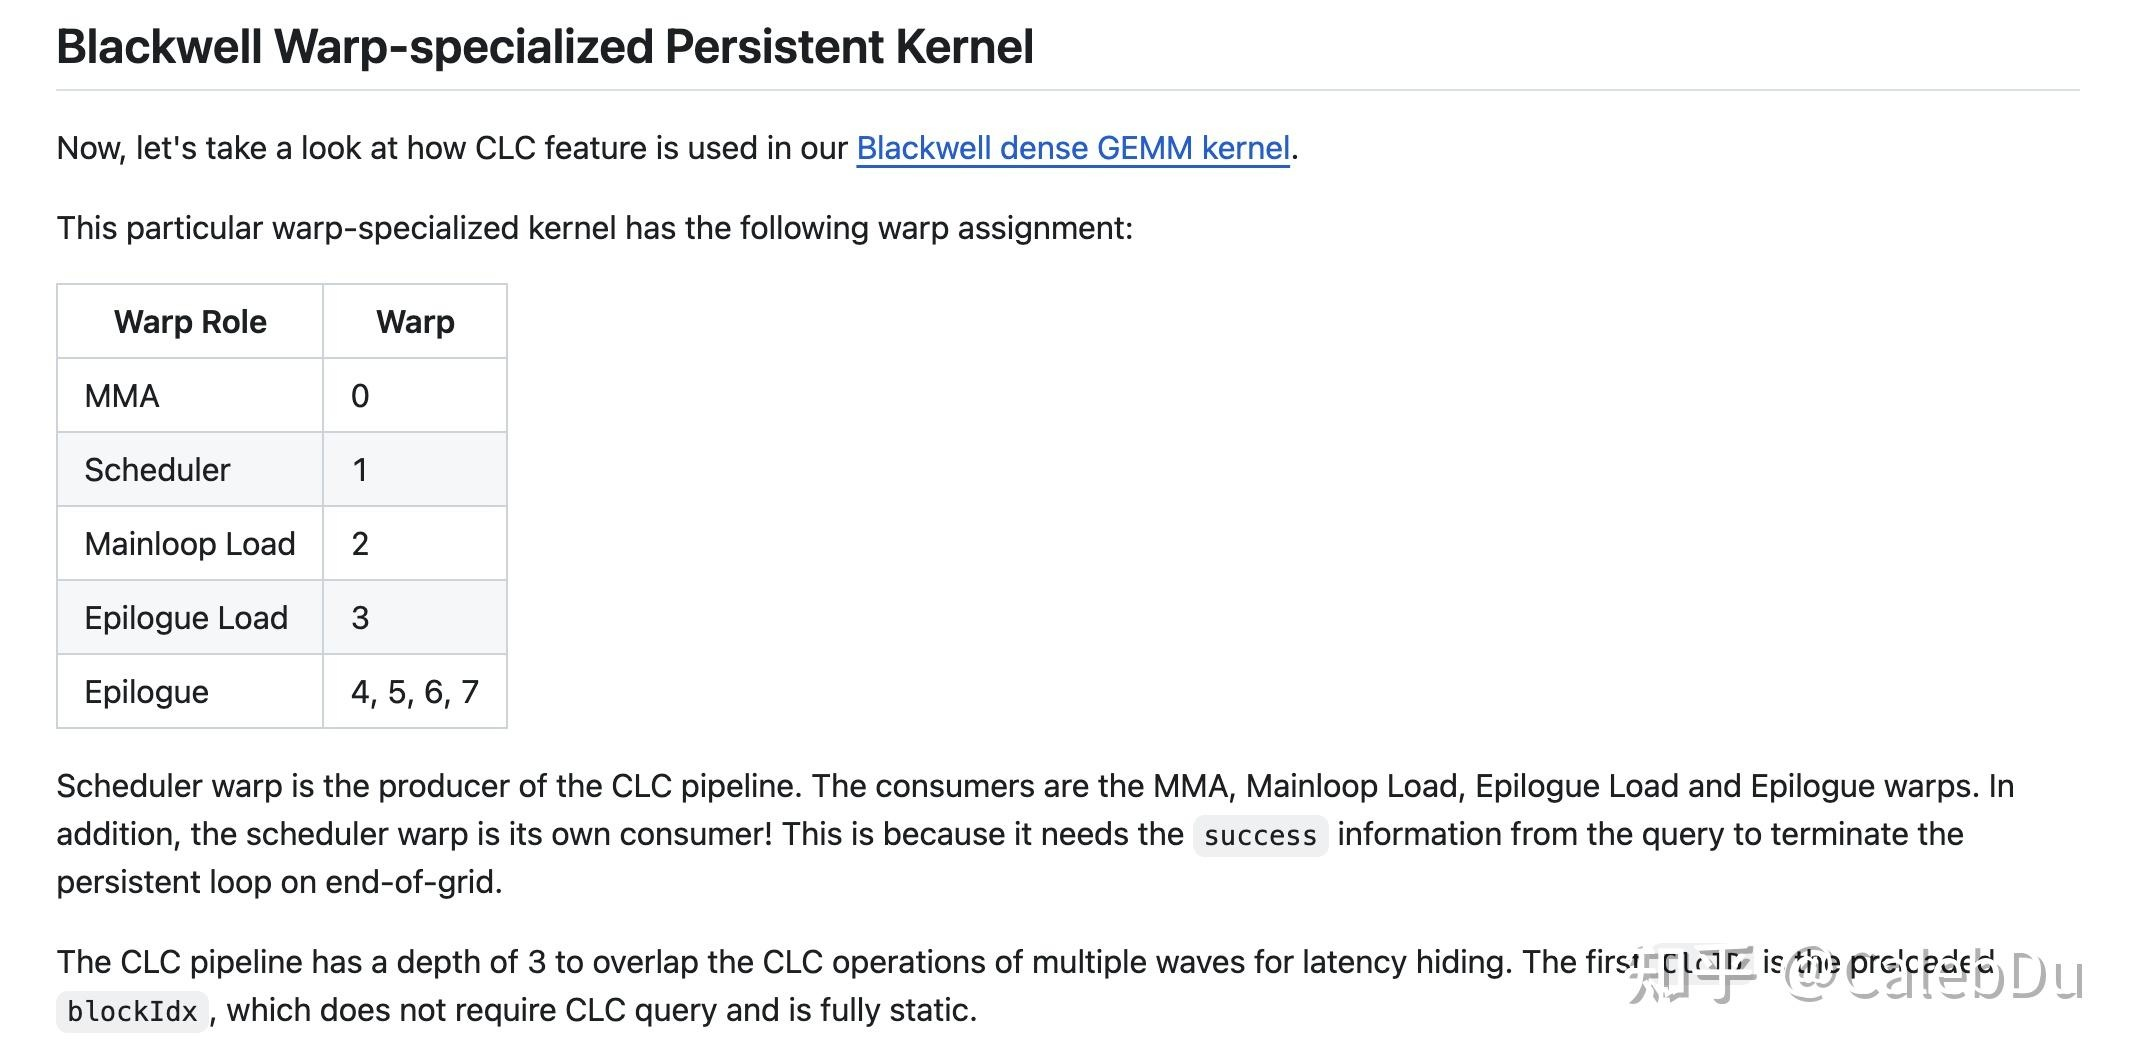
\includegraphics[width=\textwidth]{figures/calebdu-01-warp-specialization/fig-02.jpg}
\caption{warp role}
\end{figure}

在之前的文章\href{https://zhuanlan.zhihu.com/p/1940858379905001339}{Dynamic Cluster and Scheduler for Blackwell}里介绍了Blackwell 的新特性Dynamic Scheduler, scheduler warp作为生产者调用CLC ptx 指令去动态的获取后续执行的CTA id，获取到底CTA id存储在smem给所有warp进行计算next tile info。

此外， 不同于Hopper 架构的wgmma tensorcore，Blackwell 全新的\textbf{tcgen5} tensorcore指令不再需要一个warp group参与，只需要一个thread 发起tcgen5指令。同时tcgen5 的completion\_\allowbreak{}mechanism 直接由mbarrier 进行控制，不再是Hopper上调用wgmma.wait\_\allowbreak{}group 指令控制tensor core计算的完成（与mbarrier分离），这样在Blackwell上tcgen5的tensor core计算同样可以通过pipeline来控制。

\begin{figure}[H]\centering
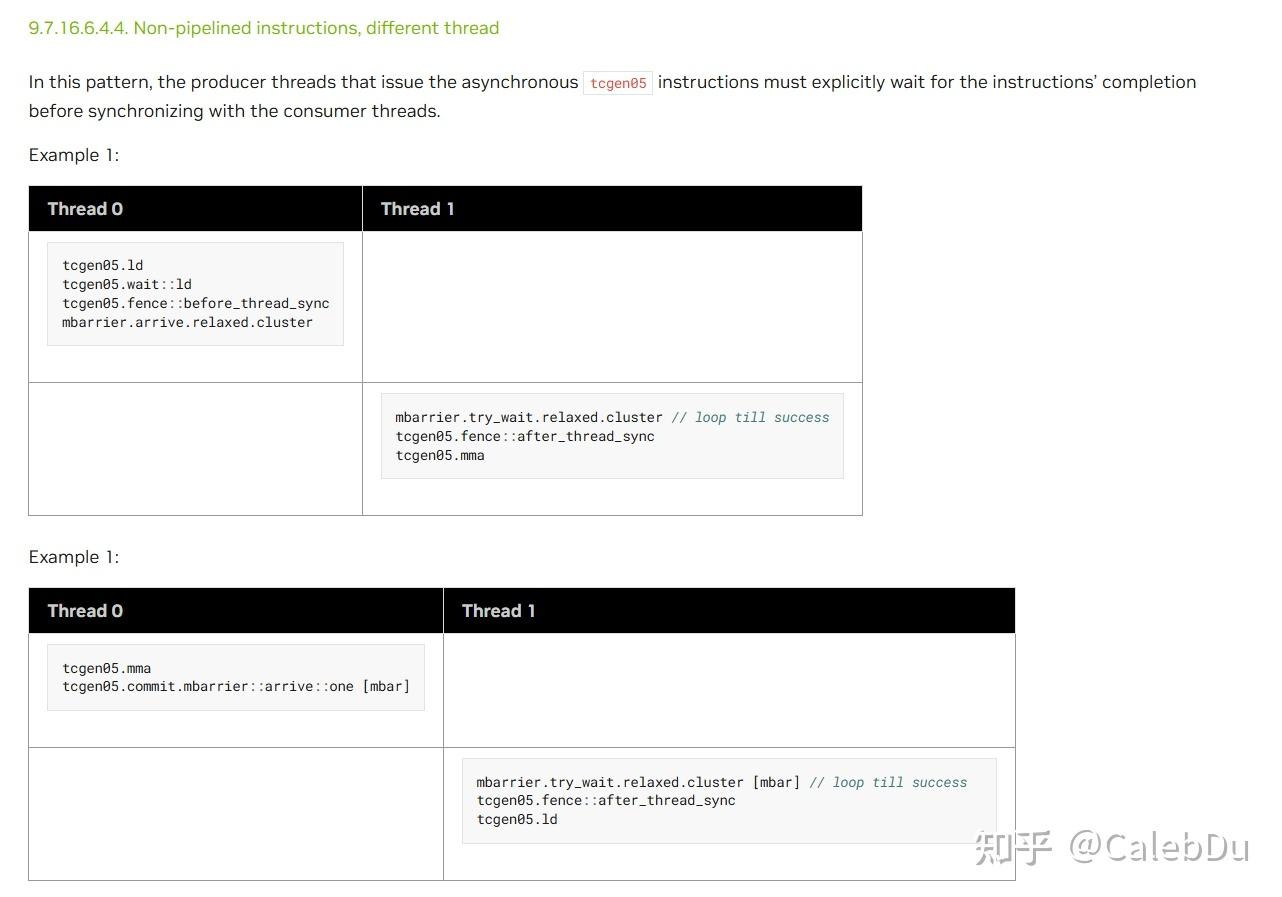
\includegraphics[width=\textwidth]{figures/calebdu-01-warp-specialization/fig-03.jpg}
\end{figure}

\begin{figure}[H]\centering
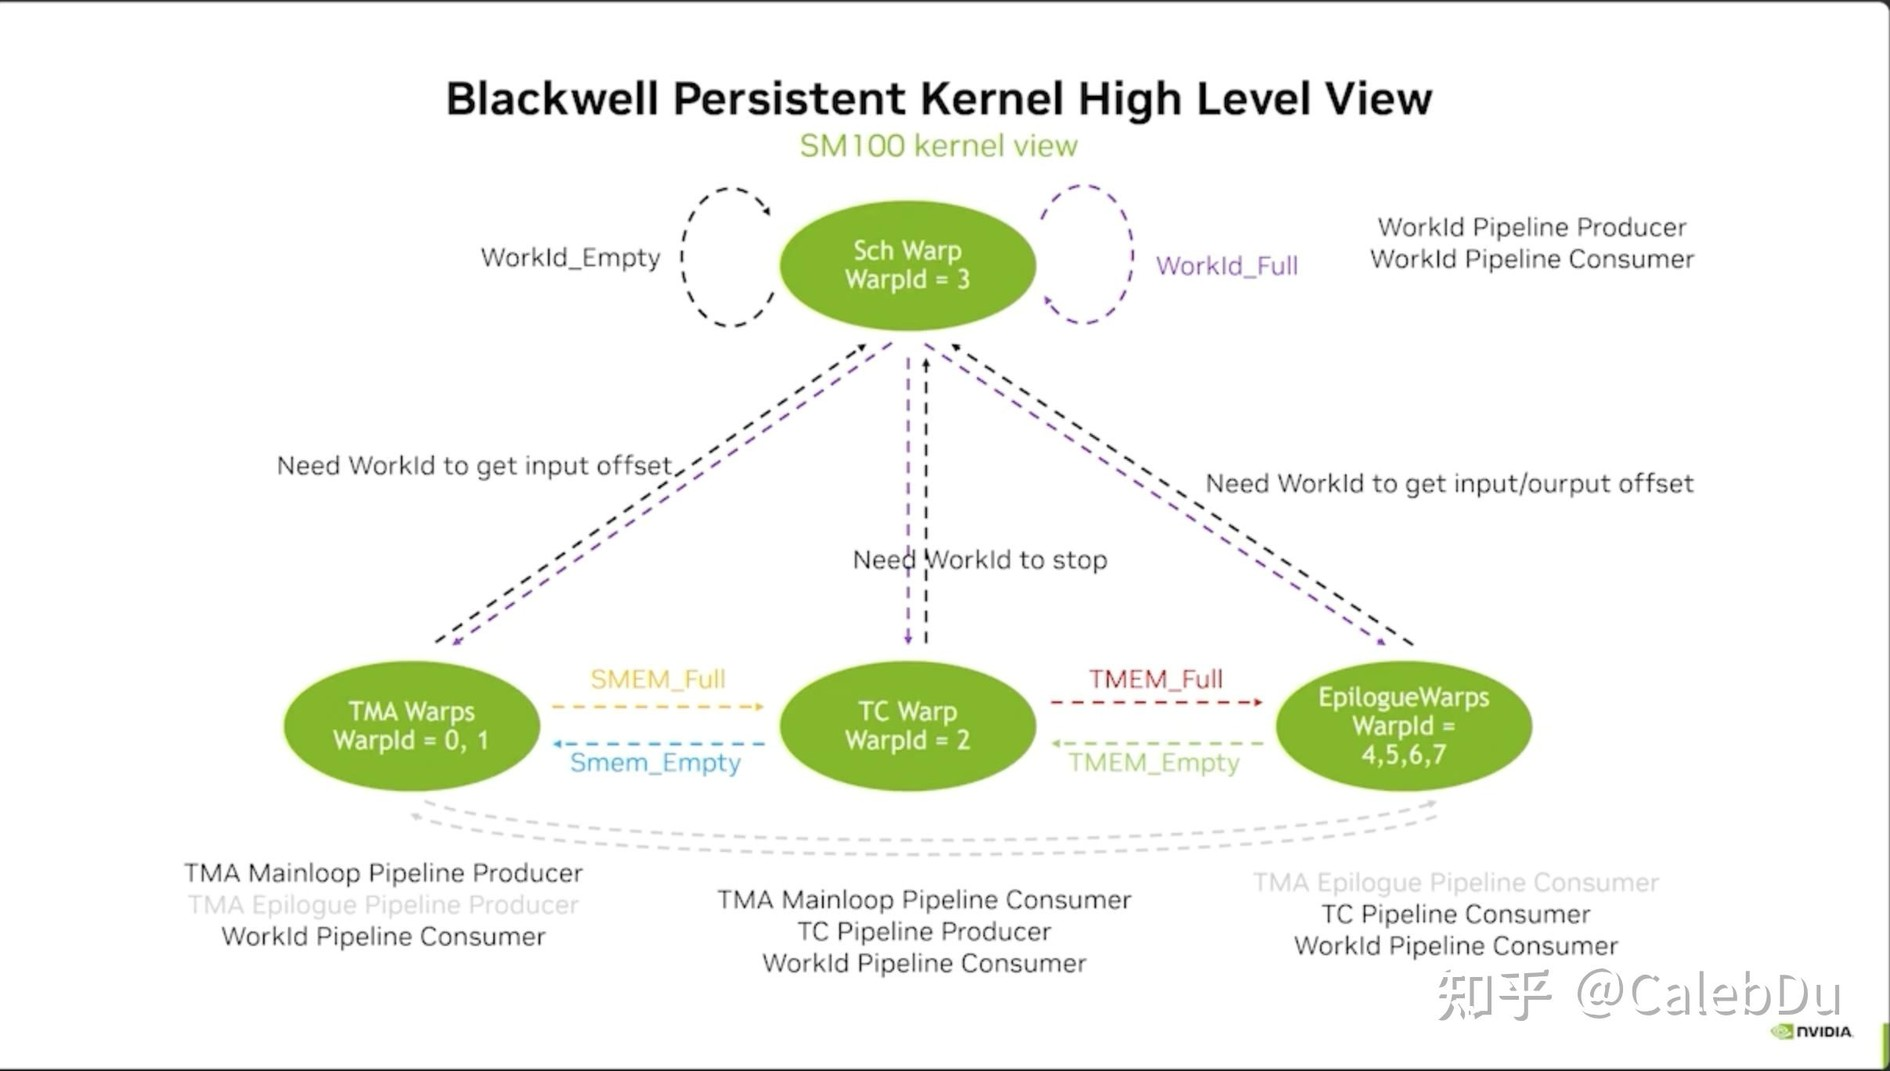
\includegraphics[width=0.9\textwidth]{figures/calebdu-01-warp-specialization/fig-04.jpg}
\caption{\url{https://www.bilibili.com/video/BV11tMwznEmo}}
\end{figure}

在Blackwell上WASP需要以下的Pipeline，来进行不同warp之间的同步

\begin{itemize}
\item \textbf{mainloop\_\allowbreak{}pipeline:}负责mainloop 数据搬运和计算之间的同步,生产者:main load warp,消费者:mma warp
\item \textbf{epilog\_\allowbreak{}load\_\allowbreak{}pipeline:}负责epilog 数据搬运和计算之间的同步,生产者:epilog load warp,消费者:epilog warp
\item \textbf{clc\_\allowbreak{}pipeline:}负责CLC response的获取和对应tile info的计算,生产者:scheduler warp,消费者:所有 warp
\item \textbf{clc\_\allowbreak{}throttle\_\allowbreak{}pipeline:}控制scheduler warp 的调度下一个tile的速度,防止tile info 踩踏，生产者:main load warp,消费者:scheduler warp
\item \textbf{accumulator\_\allowbreak{}pipeline:}负责tcgen5 mma结果的完成和epilog 计算之间的同步,生产者: mma warp,消费者:epilog warp
\item \textbf{load\_\allowbreak{}order\_\allowbreak{}pipeline:}保证prolog第一个tile mainloop load之后，再发射epilog load
\end{itemize}

\begin{figure}[H]\centering
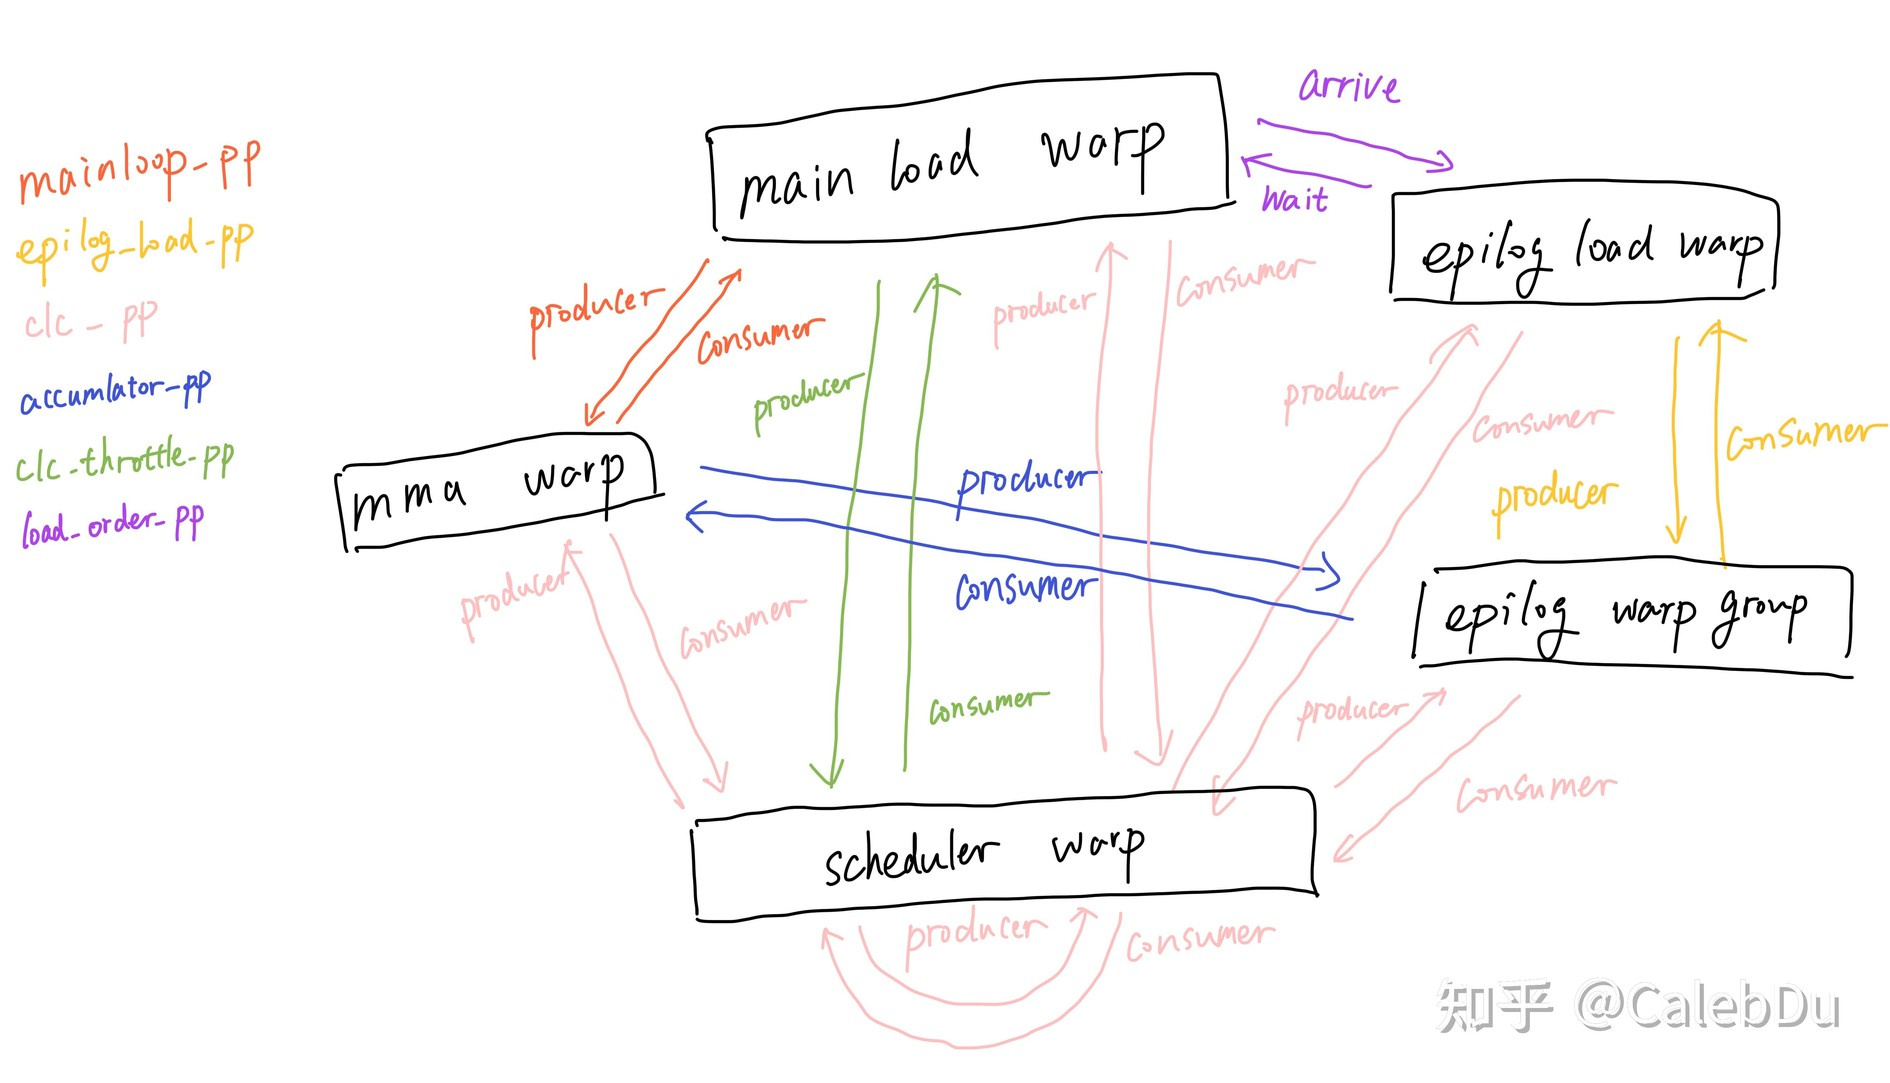
\includegraphics[width=0.9\textwidth]{figures/calebdu-01-warp-specialization/fig-05.jpg}
\end{figure}

下图简单的画了Blackwell WASP 不同的warp如何基于pipeline进行通信实现同步，图中的缩写代表producer\_\allowbreak{}acquire(\textbf{PA}), producer\_\allowbreak{}commit(\textbf{PC}),consumer\_\allowbreak{}wait(\textbf{CW),}consumer\_\allowbreak{}release(\textbf{CR}), mbar(\textbf{mbar\_\allowbreak{}expect\_\allowbreak{}tx,}TMA pipeline 不需要调用\textbf{PC}), 虚线的PA 代表最初的pipeline state \textbf{phase=1} 第一次wait不触发。

\begin{figure}[H]\centering
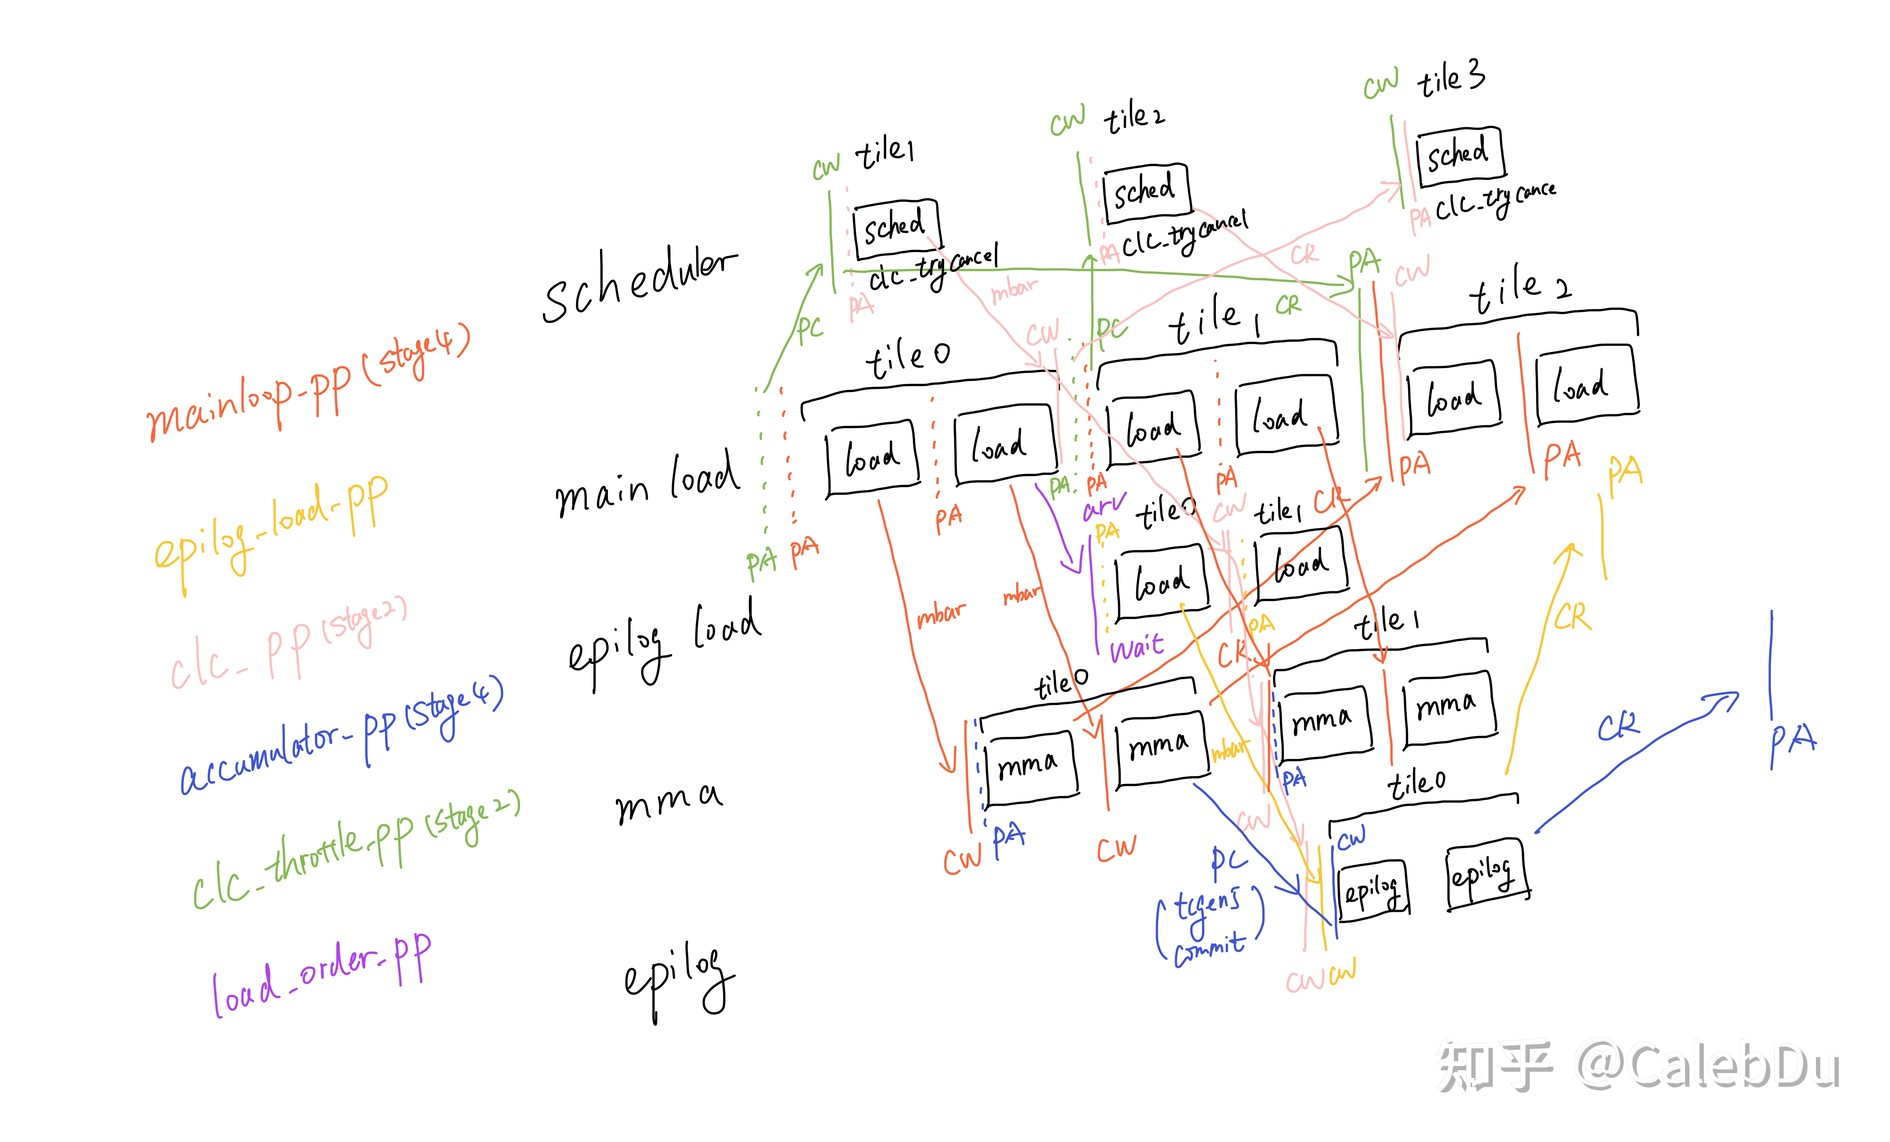
\includegraphics[width=0.9\textwidth]{figures/calebdu-01-warp-specialization/fig-06.jpg}
\end{figure}

\begin{figure}[H]\centering
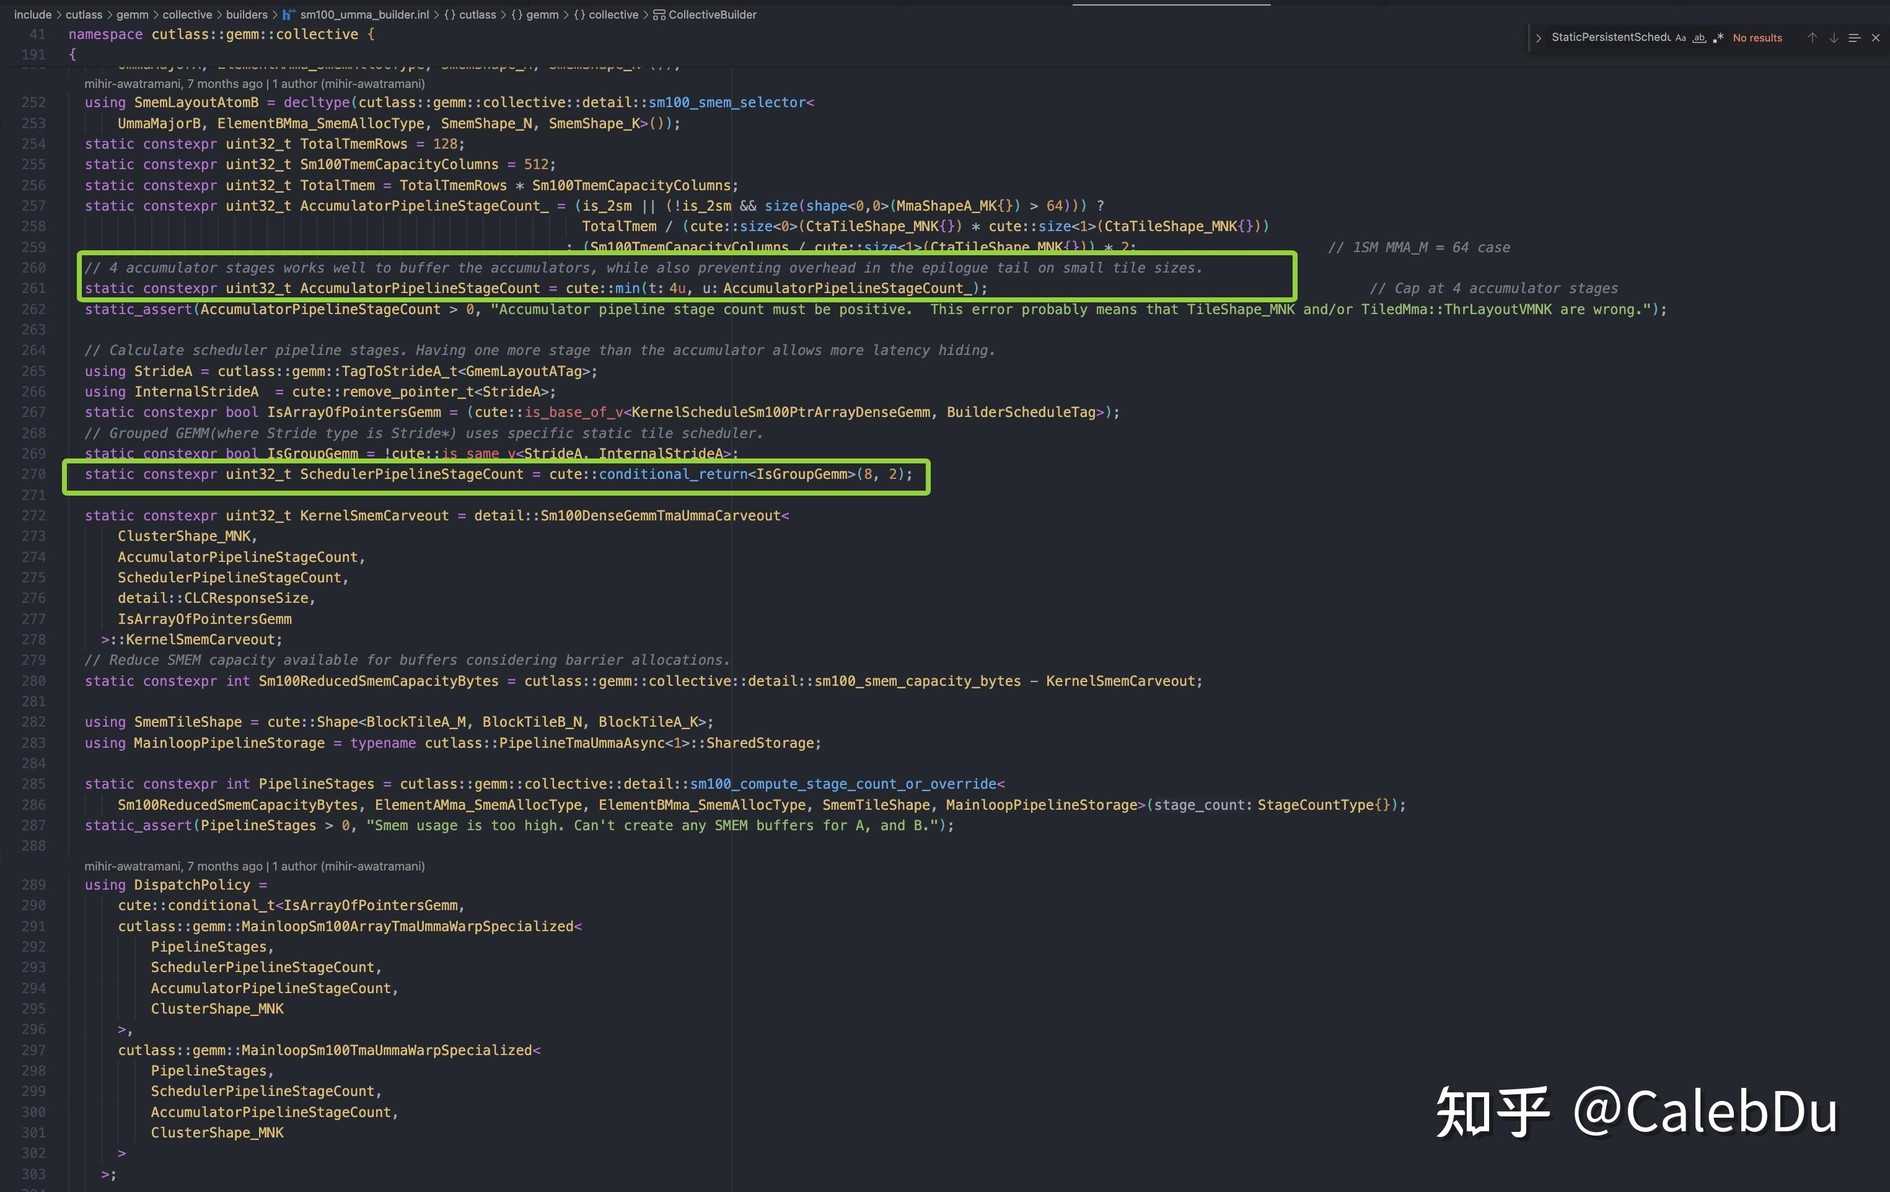
\includegraphics[width=0.9\textwidth]{figures/calebdu-01-warp-specialization/fig-07.jpg}
\caption{gemm::\allowbreak{}Collective\allowbreak{}Builder}
\end{figure}

include/\allowbreak{}cutlass/\allowbreak{}pipeline/\allowbreak{}sm100\_\allowbreak{}pipeline.hpp 基于include/\allowbreak{}cutlass/\allowbreak{}pipeline/\allowbreak{}sm90\_\allowbreak{}pipeline.hpp 中的pipeline，针对blackwell的场景，封装了新的pipeline， 如\textbf{Pipeline\allowbreak{}Umma\allowbreak{}Async}(继承Pipeline\allowbreak{}Async, \textbf{tcgen5.commit}重载producer\_\allowbreak{}commit，用于accumulator\_\allowbreak{}pipeline) , \textbf{Pipeline\allowbreak{}Tma\allowbreak{}Umma\allowbreak{}Async}(继承Pipeline\allowbreak{}Tma\allowbreak{}Async, \textbf{tcgen5.commit} 重载consumer\_\allowbreak{}release，用于mainloop\_\allowbreak{}pipeline), \textbf{Pipeline\allowbreak{}CLCFetch\allowbreak{}Async(}用于clc\_\allowbreak{}pipeline)

\section{总结}

随着GPU引入越来越多DSA的特性，为了达到最佳的SOL性能，需要引入更复杂的pipeline来尽可能隐藏延迟和打满计算单元的吞吐。基于WASP的异步编程与pipeline通信是未来GPU获得最优性能的必要手段。

\endgroup
